% =============================================================================
\section{Instalar todo con vespo}
% =============================================================================

% La barra de pasos de arriba de cada lámina de esta sección: \camino{n} resalta el paso n.
\newcommand{\camino}[1]{%
  \begin{tikzpicture}[every node/.style={font=\tiny}]
    \foreach \i/\t in {1/clonar,2/bootstrap,3/init,4/doctor,5/build,6/up,7/ejemplo,8/down} {
      \ifnum\i<#1 \def\cc{verde}\def\ff{verde!20}\else\ifnum\i=#1 \def\cc{azul}\def\ff{yellow!50}\else\def\cc{gray!60}\def\ff{white}\fi\fi
      \node[circle,draw=\cc,fill=\ff,line width=0.8pt,minimum size=0.42cm,font=\tiny\bfseries] (c\i) at (\i*1.62,0) {\i};
      \node[below=0.02cm of c\i,text=\cc] {\t};
      \ifnum\i>1 \pgfmathtruncatemacro{\p}{\i-1}\draw[gray!60] (c\p) -- (c\i);\fi
    }
  \end{tikzpicture}\par\vspace{0.2em}}

\begin{frame}{El camino completo}
  \centering
  \begin{tikzpicture}[every node/.style={font=\scriptsize,align=center},
      st/.style={draw=azul,fill=azulclaro,rounded corners,minimum width=2.6cm,minimum height=1.25cm,text width=2.5cm}]
    \node[st] (a) at (0,1.6) {\textbf{1 Clonar}\\\cmd{git clone}\\una sola vez};
    \node[st] (b) at (3.4,1.6) {\textbf{2 bootstrap}\\instala ROS 2\\y \cmd{vespo}};
    \node[st] (c) at (6.8,1.6) {\textbf{3 vespo init}\\PX4, Gazebo, QGC\\y compila};
    \node[st] (d) at (10.2,1.6) {\textbf{4 vespo doctor}\\¿todo en orden?};
    \node[st,fill=yellow!25] (e) at (10.2,-0.6) {\textbf{5 vespo build}\\cuando cambias\\código};
    \node[st,fill=yellow!25] (f) at (6.8,-0.6) {\textbf{6 vespo up -{}-sim}\\levanta la\\simulación};
    \node[st,fill=yellow!25] (g) at (3.4,-0.6) {\textbf{7 ros2 run}\\corre un\\ejemplo};
    \node[st,fill=yellow!25] (h) at (0,-0.6) {\textbf{8 vespo down}\\apaga todo};
    \draw[-{Stealth},thick] (a) -- (b); \draw[-{Stealth},thick] (b) -- (c); \draw[-{Stealth},thick] (c) -- (d);
    \draw[-{Stealth},thick] (d) -- (e); \draw[-{Stealth},thick] (e) -- (f); \draw[-{Stealth},thick] (f) -- (g);
    \draw[-{Stealth},thick] (g) -- (h);
    \draw[decorate,decoration={brace,amplitude=5pt,mirror},gris] (-1.3,0.5) -- (-1.3,2.7)
      node[midway,left=6pt,font=\tiny,text=gris] {una vez};
    \draw[decorate,decoration={brace,amplitude=5pt},gris] (11.5,0.0) -- (11.5,-1.2)
      node[midway,right=6pt,font=\tiny,text=gris,text width=1.3cm] {cada día};
  \end{tikzpicture}
  \vspace{0.5em}

  \raggedright\small Los pasos \textbf{1 a 4} se hacen una vez por computadora. Del \textbf{5 al 8} es lo de
  todos los días.
\end{frame}

\begin{frame}{Antes de empezar}
  \camino{0}
  \begin{columns}[t]
    \column{0.48\textwidth}
    \begin{idea}[title={\small\bfseries Lo que necesitas},coltitle=black,colbacktitle=azulclaro]
      \small
      \begin{itemize}
        \item \textbf{Ubuntu 24.04} (no otra versión: es la única con ROS 2 Jazzy).
        \item \textbf{\textasciitilde30 GB libres}: PX4 y Gazebo solos ocupan \textasciitilde15 GB.
        \item \textbf{Buen internet}: la primera vez baja varios GB.
        \item Tu \textbf{contraseña} (pide \cmd{sudo} para instalar).
        \item \textbf{1 a 2 horas} la primera vez.
      \end{itemize}
    \end{idea}
    \column{0.48\textwidth}
    \begin{ojo}[title={\small\bfseries Conecta el cargador}]
      \small La simulación usa mucho CPU y tarjeta de video. Con batería la laptop se pone lenta y puede
      \textbf{apagarse sola} a media simulación.
    \end{ojo}
    \begin{idea}
      \small Si algo se corta (internet, batería), \textbf{no pasa nada}: vuelves a correr el mismo comando y
      sigue donde iba.
    \end{idea}
  \end{columns}
\end{frame}

\begin{frame}[fragile]{Paso 1: clonar el repositorio}
  \camino{1}
  \begin{lstlisting}[style=bash]
sudo apt install git                                   # si no lo tienes
cd ~                                                   # en tu carpeta personal
git clone https://github.com/Imcab/vespo_ws.git
cd vespo_ws
  \end{lstlisting}
  \begin{columns}[c]
    \column{0.5\textwidth}\centering
    \begin{tikzpicture}[every node/.style={font=\scriptsize,anchor=west}]
      \node at (0,2.1) {\textbf{\textasciitilde/} (tu carpeta)};
      \draw[gray] (0.2,1.85) |- (0.5,1.5); \node at (0.5,1.5) {\cmd{vespo\_ws/} \color{gris}el workspace del equipo};
      \draw[gray] (0.7,1.25) |- (1.0,0.95); \node at (1.0,0.95) {\cmd{src/} \color{gris}los paquetes de ROS 2};
      \draw[gray] (0.7,1.25) |- (1.0,0.55); \node at (1.0,0.55) {\cmd{tools/} \color{gris}el comando vespo};
      \draw[gray] (0.7,1.25) |- (1.0,0.15); \node at (1.0,0.15) {\cmd{vespo.toml} \color{gris}versiones del equipo};
      \draw[gray] (0.2,1.85) |- (0.5,-0.35); \node at (0.5,-0.35) {\cmd{PX4-Autopilot/} \color{gris}lo baja el paso 3};
    \end{tikzpicture}
    \column{0.47\textwidth}\small
    \begin{itemize}
      \item Un \textbf{workspace} es la carpeta con todos los paquetes de ROS 2 del equipo.
      \item PX4 vive \textbf{al lado}, no adentro.
      \item \cmd{vespo.toml} fija la versión de PX4 (\textbf{v1.17.0}): todos usan la misma.
    \end{itemize}
  \end{columns}
\end{frame}

\begin{frame}[fragile]{Paso 2: bootstrap.sh}
  \camino{2}
  \begin{lstlisting}[style=bash]
./bootstrap.sh            # dentro de vespo_ws; te pide tu contraseña
  \end{lstlisting}
  \centering
  \begin{tikzpicture}[every node/.style={font=\scriptsize,align=center},
      bx/.style={draw=azul,fill=azulclaro,rounded corners,minimum width=2.5cm,minimum height=1cm}]
    \node[bx,fill=gray!10,draw=gray] (u) at (0,0) {Ubuntu 24.04\\recién instalado};
    \node[bx] (r) at (3.5,0.75) {\textbf{ROS 2 Jazzy}};
    \node[bx] (t) at (3.5,-0.75) {\textbf{colcon, vcs, rosdep}\\herramientas para compilar};
    \node[bx] (v) at (7,0) {\textbf{el comando vespo}};
    \node[bx,fill=yellow!30] (i) at (10.5,0) {arranca solo\\\textbf{vespo init}};
    \draw[-{Stealth},thick] (u) -- (r); \draw[-{Stealth},thick] (u) -- (t);
    \draw[-{Stealth},thick] (r) -- (v); \draw[-{Stealth},thick] (t) -- (v); \draw[-{Stealth},thick] (v) -- (i);
  \end{tikzpicture}
  \vspace{0.6em}

  \raggedright\small
  \begin{itemize}
    \item Es lo \textbf{único} que se corre a mano en una máquina nueva: lo demás lo hace \cmd{vespo}.
    \item Al terminar le pasa el control a \cmd{vespo init} (el paso 3), que te va a hacer preguntas.
    \item Si se corta: \cmd{./bootstrap.sh} otra vez.
  \end{itemize}
\end{frame}

\begin{frame}{Paso 3: vespo init, las preguntas}
  \camino{3}
  \small \cmd{vespo init} pregunta en inglés. Para una laptop de simulación:
  \vspace{0.3em}

  \begin{columns}[t]
    \column{0.5\textwidth}
    \textbf{Primero, cómo es tu máquina}\\[0.3em]
    \scriptsize
    \begin{tabular}{@{}p{3.1cm}p{3.3cm}@{}}
      \toprule
      Te pregunta & Contesta \\
      \midrule
      \cmd{Role of this machine} & \textbf{sim} (tu laptop simula) \\
      \cmd{ROS\_DOMAIN\_ID} & \textbf{tu número} (siguiente lámina) \\
      \cmd{Flight controller} & \textbf{None yet} (no hay Pixhawk) \\
      \cmd{Path to PX4-Autopilot} & \textbf{Enter} (al lado de \cmd{vespo\_ws}) \\
      Simulation defaults & \textbf{Enter} a todo \\
      \bottomrule
    \end{tabular}
    \column{0.46\textwidth}
    \textbf{Luego, qué instalar: Y a todo}\\[0.3em]
    \scriptsize
    \begin{tabular}{@{}p{3.6cm}p{2.3cm}@{}}
      \toprule
      Te pregunta & Hace \\
      \midrule
      \cmd{Clone them now with vcs?} & baja \cmd{px4\_msgs} y el agente \\
      \cmd{Install them now in \ldots?} & PX4 y Gazebo, \textbf{\textasciitilde15 GB} \\
      \cmd{Install missing ROS dependencies\ldots?} & pide contraseña \\
      \cmd{Build the workspace now?} & compila \\
      \cmd{Build PX4 SITL now?} & compila PX4 \\
      \cmd{Download QGroundControl now?} & la estación de tierra \\
      \cmd{Add vespo\ldots{} to \textasciitilde/.bashrc?} & cada terminal lo tiene \\
      \bottomrule
    \end{tabular}
  \end{columns}
  \vspace{0.4em}
  \small Termina con \cmd{sim machine ready}. Si lo vuelves a correr, tus respuestas anteriores salen por defecto.
\end{frame}

\begin{frame}{ROS\_DOMAIN\_ID: cada quien su canal}
  \camino{3}
  \begin{columns}[c]
    \column{0.55\textwidth}\centering
    \begin{tikzpicture}[every node/.style={font=\scriptsize,align=center}]
      \node[draw=gray,fill=gray!10,rounded corners,minimum width=5.6cm,minimum height=0.6cm] (w) at (0,0) {la misma red WiFi};
      \node[draw=azul,fill=azulclaro,rounded corners] (a) at (-2,1.5) {laptop de Ana\\ID 0};
      \node[draw=azul,fill=azulclaro,rounded corners] (b) at (2,1.5) {laptop de Beto\\ID 0};
      \draw[thick] (a) -- (w); \draw[thick] (b) -- (w);
      \node[text=rojo,font=\scriptsize\bfseries] at (0,1.5) {¡se mezclan!};
      \node[draw=azul,fill=azulclaro,rounded corners] (c) at (-2,-1.5) {laptop de Ana\\ID 7};
      \node[draw=azul,fill=azulclaro,rounded corners] (d) at (2,-1.5) {laptop de Beto\\ID 12};
      \draw[thick] (c) -- (w); \draw[thick] (d) -- (w);
      \node[text=verde,font=\scriptsize\bfseries] at (0,-1.5) {separados};
    \end{tikzpicture}
    \column{0.42\textwidth}\small
    \begin{itemize}
      \item En la misma red, los nodos de ROS 2 de \textbf{distintas laptops se ven entre sí}.
      \item Si dos personas simulan con el mismo ID, tu nodo puede leer (\textbf{y mandarle órdenes}) al dron
        de otro.
      \item Cada quien usa \textbf{su número} (0 a 232).
      \item Cambiarlo después: \cmd{vespo config edit domain\_id}.
    \end{itemize}
  \end{columns}
\end{frame}

\begin{frame}[fragile]{Paso 4: terminal nueva y vespo doctor}
  \camino{4}
  \begin{columns}[t]
    \column{0.45\textwidth}
    \begin{lstlisting}[style=bash]
# abre una terminal NUEVA (la vieja
# todavia no conoce el comando vespo)
vespo doctor
    \end{lstlisting}
    \small Revisa todo lo que se instaló y te dice si falta algo. Úsalo \textbf{siempre que algo no
    funcione}: es lo primero.
    \vspace{0.4em}
    \begin{idea}
      \small Junto a cada \textcolor{rojo}{\ding{55}} viene un \cmd{fix:} con el comando que lo arregla.
    \end{idea}
    \column{0.52\textwidth}
    \begin{terminal}{vespo doctor}
System ──────────────────────\\
{\color{verde}✔} ROS 2 jazzy installed\\
{\color{verde}✔} colcon found\\
Workspace ───────────────────\\
{\color{verde}✔} Role: sim\\
{\color{verde}✔} px4\_msgs at the pinned version\\
PX4 ─────────────────────────\\
{\color{verde}✔} PX4-Autopilot at v1.17.0\\
{\color{verde}✔} px4\_msgs matches PX4's messages\\
{\color{verde}✔} PX4 SITL built\\
{\color{verde}✔} Gazebo Harmonic 8.15.0\\
Link to PX4 ─────────────────\\
{\color{verde}✔} UDP port 8888 free\\
QGroundControl ──────────────\\
{\color{verde}✔} Installed at \ldots/QGroundControl\ldots\\[0.3em]
{\color{verde}✔} All good
    \end{terminal}
  \end{columns}
\end{frame}

\begin{frame}{Si doctor marca algo en rojo}
  \camino{4}
  \centering\scriptsize
  \begin{tabular}{p{5.3cm}p{3.3cm}p{4.6cm}}
    \toprule
    Dice & Corre & Qué pasó \\
    \midrule
    \cmd{PX4-Autopilot is not at the pinned v1.17.0} & \cmd{vespo px4 sync} & PX4 en otra versión (p.\,ej. clonado de
      \cmd{main}) \\
    \cmd{px4\_msgs differs from PX4} & \cmd{vespo px4 sync} & los mensajes no coinciden: los topics llegarían mal \\
    \cmd{px4\_msgs not built} & \cmd{vespo build} & falta compilar \\
    \cmd{px4\_msgs not cloned} & \cmd{vespo init} & se saltó la clonada \\
    \cmd{Workspace not in \textasciitilde/.bashrc} & \cmd{vespo init} & contestaste \textbf{n} a la última pregunta \\
    \cmd{ROS\_DOMAIN\_ID is \ldots{} in this shell} & abre otra terminal & la terminal es de antes del cambio \\
    \cmd{UDP port 8888 busy} & \cmd{vespo down} & quedó un agente corriendo \\
    \cmd{QGroundControl: Not installed} & \cmd{vespo qgc install} & no se bajó QGC \\
    \bottomrule
  \end{tabular}
  \vspace{0.5em}

  \raggedright\small Ninguna de estas se arregla reinstalando todo: corre el \cmd{fix} que dice y vuelve a
  correr \cmd{vespo doctor}.
\end{frame}

\begin{frame}[fragile]{Paso 5: vespo build}
  \camino{5}
  \begin{lstlisting}[style=bash]
vespo build                    # todo el workspace
vespo build px4_examples       # solo un paquete (mucho mas rapido)
  \end{lstlisting}
  \begin{columns}[c]
    \column{0.52\textwidth}\centering
    \begin{tikzpicture}[every node/.style={font=\scriptsize,align=center},
        bx/.style={draw=azul,fill=azulclaro,rounded corners,minimum width=2.2cm,minimum height=0.9cm}]
      \node[bx] (s) at (0,0) {\cmd{src/}\\tu código .cpp};
      \node[bx,fill=yellow!25] (c) at (2.9,0) {\textbf{colcon}\\compila};
      \node[bx] (i) at (5.8,0) {\cmd{install/}\\los programas};
      \node[draw=gray,fill=gray!10,rounded corners] (r) at (5.8,-1.4) {\cmd{ros2 run} los\\busca aquí};
      \draw[-{Stealth},thick] (s) -- (c); \draw[-{Stealth},thick] (c) -- (i); \draw[-{Stealth},thick] (r) -- (i);
    \end{tikzpicture}
    \column{0.45\textwidth}\small
    \textbf{¿Cuándo?}
    \begin{itemize}
      \item Cada vez que \textbf{cambias un .cpp}: C++ no corre el código nuevo hasta compilarlo.
      \item Después de \cmd{vespo update} no hace falta: ya compila solo lo que cambió.
    \end{itemize}
  \end{columns}
  \begin{ojo}
    \small ¿Cambiaste el código y el dron hace lo mismo de antes? Casi siempre es que \textbf{no compilaste}, o
    que el build falló y no viste el error.
  \end{ojo}
\end{frame}

\begin{frame}[fragile]{Paso 6: vespo up -{}-sim}
  \camino{6}
  \begin{columns}[c]
    \column{0.5\textwidth}
    \begin{lstlisting}[style=bash]
vespo up --sim
    \end{lstlisting}
    \centering
    \begin{tikzpicture}[every node/.style={font=\scriptsize,align=center},
        bx/.style={draw=azul,fill=azulclaro,rounded corners,minimum width=2.4cm,minimum height=0.85cm}]
      \node[bx,fill=yellow!30] (v) at (0,0) {\textbf{vespo up -{}-sim}};
      \node[bx] (a) at (-2.2,-1.5) {\textbf{agente}\\el traductor};
      \node[bx] (p) at (0.4,-1.5) {\textbf{PX4 + Gazebo}\\el dron y el mundo};
      \node[bx] (q) at (3.0,-1.5) {\textbf{QGroundControl}\\la torre};
      \foreach \n in {a,p,q} \draw[-{Stealth},thick] (v) -- (\n);
    \end{tikzpicture}
    \vspace{0.3em}

    \raggedright\small Espera a que QGC diga \textbf{Ready To Fly} (\textasciitilde30 s).
    \column{0.47\textwidth}\centering
    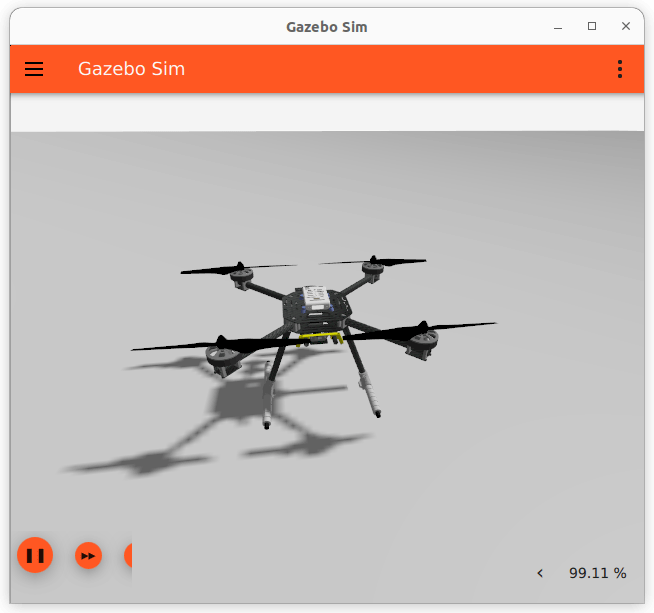
\includegraphics[height=0.42\textheight]{gazebo_x500}\\
    \credito{Gazebo con el x500. Documentación de PX4 (CC BY 4.0)}
  \end{columns}
  \vspace{0.2em}
  \begin{idea}
    \small En la terminal \textbf{kitty} cada programa sale en su propio panel. En otra terminal salen todos
    juntos, cada línea con el nombre del programa al inicio. \textbf{Ctrl+C} los para a todos.
  \end{idea}
\end{frame}

\begin{frame}[fragile]{Variantes de vespo up}
  \camino{6}
  \begin{lstlisting}[style=bash]
vespo up --sim --world plaza_show                # en otro mundo (los de x500_retos)
vespo up --sim --custom x500_lidar_2d            # con otro modelo de dron
vespo up --sim --world cueva --custom x500_lidar_2d
vespo up --sim --headless                        # sin ventana de Gazebo (mas ligero)
vespo simulate --show                            # que modelos y mundos hay
  \end{lstlisting}
  \begin{columns}[c]
    \column{0.32\textwidth}\centering
    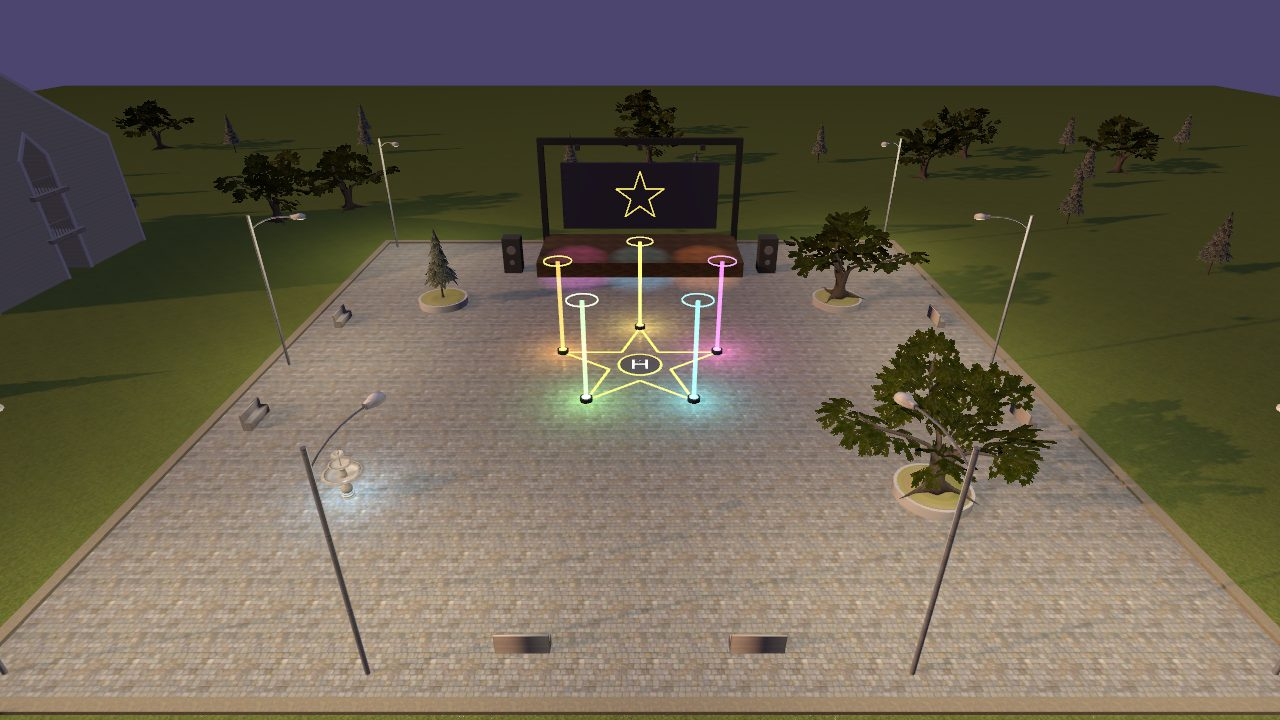
\includegraphics[width=\linewidth]{plaza_show}\\\credito{plaza\_show}
    \column{0.32\textwidth}\centering
    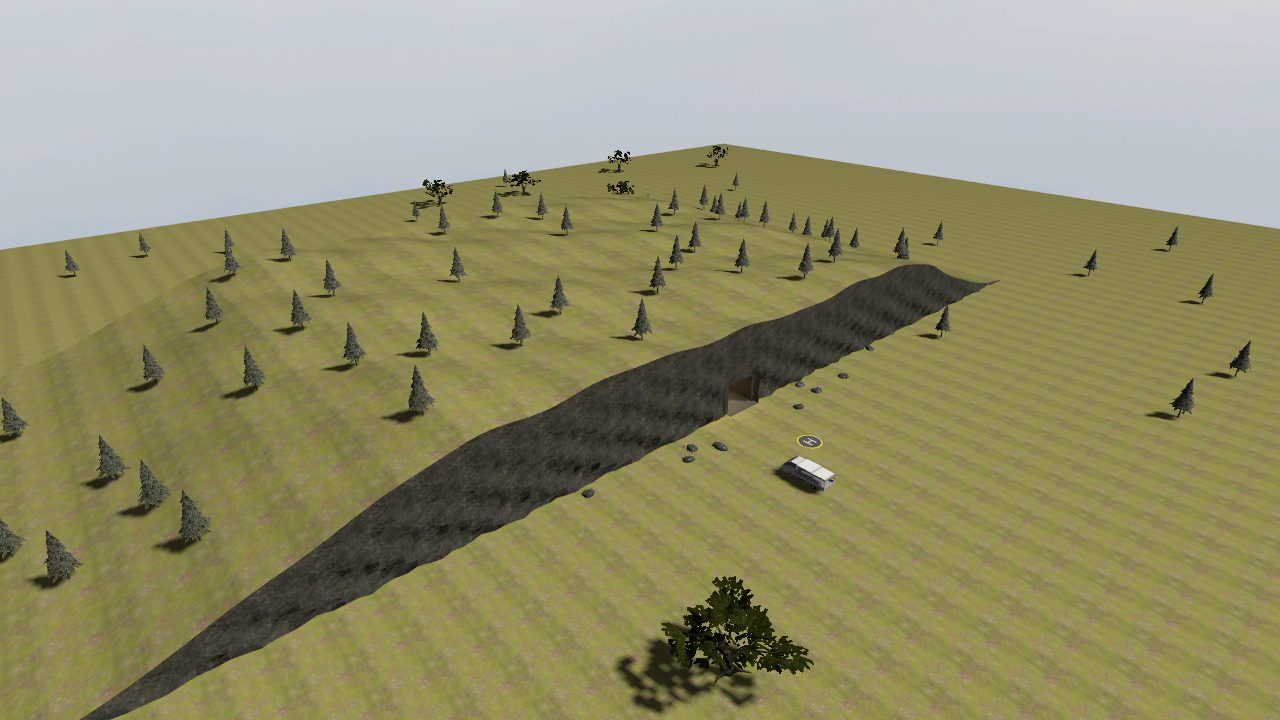
\includegraphics[width=\linewidth]{cueva}\\\credito{cueva}
    \column{0.32\textwidth}\centering
    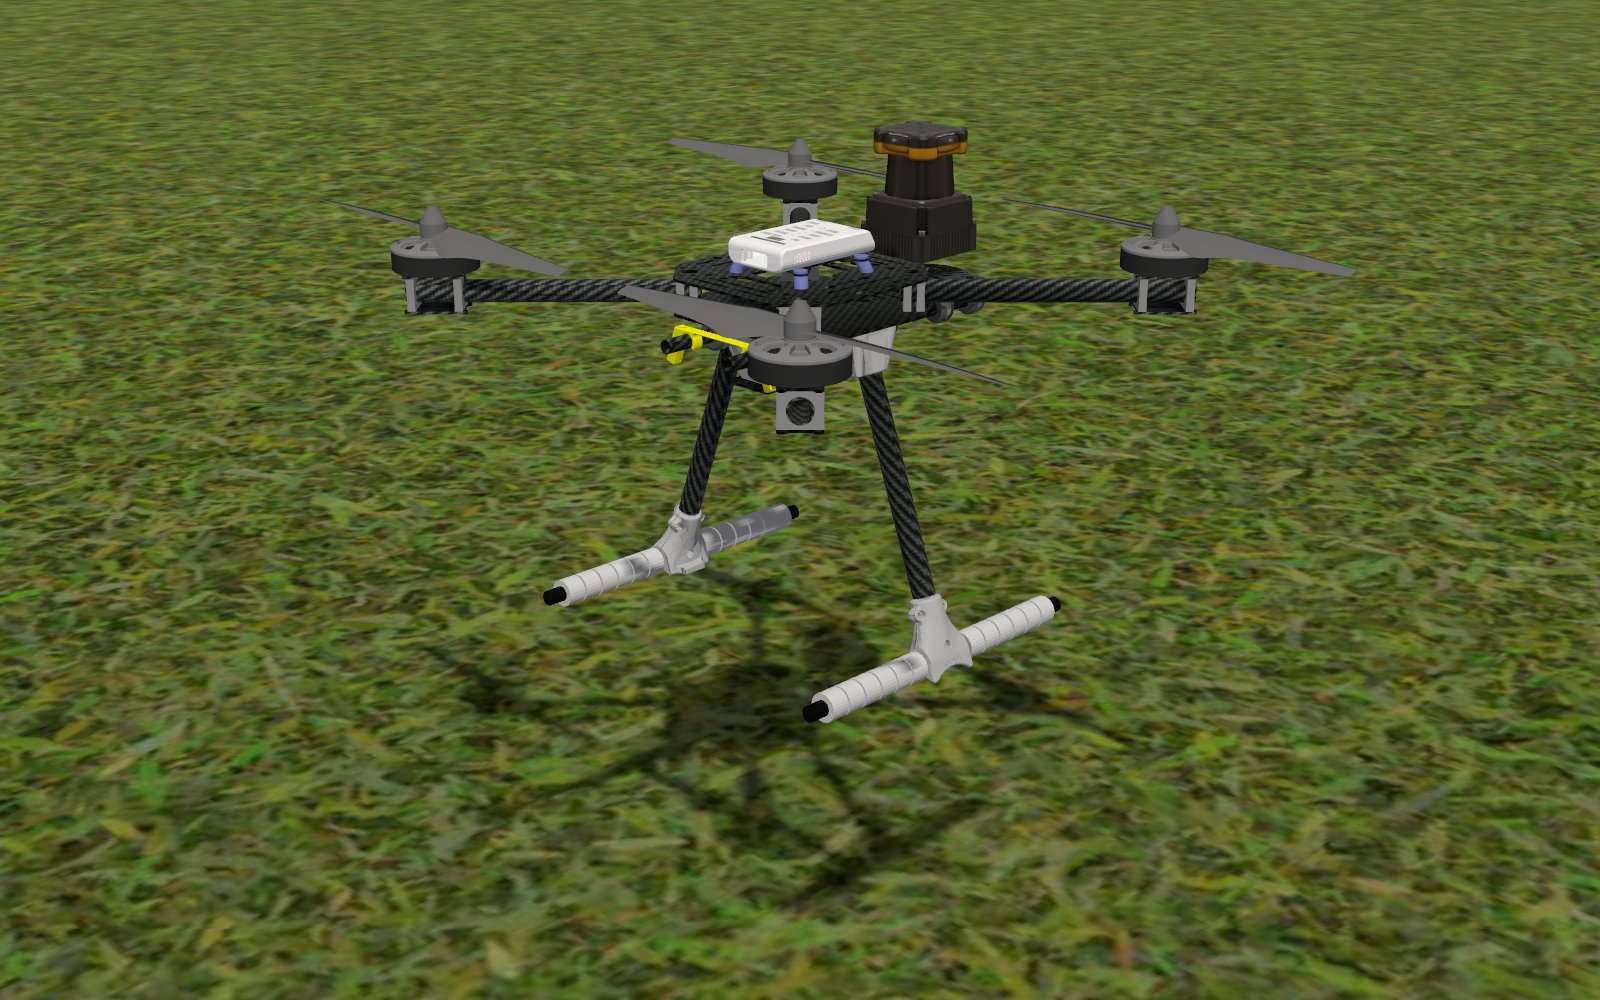
\includegraphics[width=\linewidth]{x500_lidar}\\\credito{x500\_lidar\_2d}
  \end{columns}
\end{frame}

\begin{frame}[fragile]{Paso 7: correr un ejemplo}
  \camino{7}
  \begin{columns}[c]
    \column{0.5\textwidth}
    \begin{lstlisting}[style=bash]
# en OTRA terminal (vespo up sigue corriendo)
ros2 run px4_examples telemetry_listener
    \end{lstlisting}
    \small
    \begin{itemize}
      \item \cmd{ros2 run \textit{paquete} \textit{programa}}.
      \item Tab completa los nombres: \cmd{ros2 run px4\_examples <Tab><Tab>} lista los 18 ejemplos.
      \item Lo paras con \textbf{Ctrl+C}.
    \end{itemize}
    \column{0.47\textwidth}
    \begin{terminal}{ros2 run px4\_examples telemetry\_listener}
Estado: desarmado | modo: HOLD (4)\\
Local: x=0.01 y=-0.02 alt=0.03 m\\
\ \ | vel=(0.00, 0.00, 0.00) m/s\\
GPS: lat=47.3979711 lon=8.5461637\\
Actitud: roll=0.1° pitch=-0.2° yaw=90.0°\\
Batería: 16.20 V | 100 \%
    \end{terminal}
    \small Si ves esto, \textbf{todo funciona}: ROS 2 ya habla con PX4.
  \end{columns}
\end{frame}

\begin{frame}[fragile]{Paso 8: apagar}
  \camino{8}
  \begin{columns}[c]
    \column{0.5\textwidth}
    \begin{lstlisting}[style=bash]
vespo down        # desde cualquier terminal
    \end{lstlisting}
    \small
    \begin{itemize}
      \item Para todo lo que levantó \cmd{vespo up}, y cualquier PX4, Gazebo o agente que haya quedado
        prendido.
      \item Úsalo también si la simulación se trabó: después \cmd{vespo up -{}-sim} otra vez.
    \end{itemize}
    \column{0.47\textwidth}
    \begin{ojo}[title={\small\bfseries Procesos zombis}]
      \small Si cierras la ventana de la terminal en vez de Ctrl+C, Gazebo o PX4 pueden quedarse corriendo
      escondidos. El siguiente \cmd{vespo up} choca con ellos (``port 8888 busy''). \cmd{vespo down} los
      limpia.
    \end{ojo}
  \end{columns}
\end{frame}

\begin{frame}[fragile]{El día a día}
  \begin{columns}[c]
    \column{0.55\textwidth}
    \begin{lstlisting}[style=bash]
vespo update                 # lo nuevo del equipo
vespo up --sim               # terminal 1
ros2 run px4_examples ...    # terminal 2
# ... editas un .cpp ...
vespo build px4_examples     # terminal 2
ros2 run px4_examples ...    # otra vez
vespo down                   # al terminar
    \end{lstlisting}
    \column{0.42\textwidth}\small
    \begin{itemize}
      \item \cmd{vespo} te \textbf{avisa solo} cuando el equipo subió algo nuevo.
      \item No hace falta reiniciar la simulación para probar otra versión de tu nodo: Ctrl+C al nodo,
        compilas y lo corres de nuevo.
      \item \cmd{vespo config}: ver la configuración de tu máquina.
    \end{itemize}
  \end{columns}
\end{frame}
